\chapter{BLE radio propagation}
\label{chap:rss}
\newcommand{\packetlosscell}[1]{& \footnotesize{#1}}

In order to develop a \BLE positioning system, it is beneficial, maybe even essential, to understand the behaviour of BLE radio signals.

When a wireless signal moves in an ideal environment, one can use the received signal strength (RSS) (or more precisely the loss of signal strength, or path-loss) to determine the distance between sender and receiver.
The signal power decreases quadratically with the distance; because RSS is measured in decibel, a logarithmic scale, this means that every doubling of distance leads to a signal that is approximately 6dB weaker.
When the signal strength from the sender is known (either because the sender advertises its transmit power as part of its advertising packet, or this information has been retrieved from somewhere else), the distance to the sender can be calculated.
Therefore, using the RSS of multiple transmitters is a good property to use to determine position in an ideal environment.

However, in practical indoor positioning situations, there are a number of factors influencing RSS, which have to be taken into account if RSS is to be used for positioning.
In this chapter I discuss several.

\section{Three advertising channels, three frequencies}

\fig{\gnuplot{rss}{channels}{BLE frequency, with three advertising channels}}


\fig{
    \begin{subfigure}[b]{0.5\textwidth}
        \gnuplotscale{rss}{frequency-difference-20-14-0x10}{Beacon 1 at location A}{0.55}
    \end{subfigure}
    \begin{subfigure}[b]{0.5\textwidth}
        \gnuplotscale{rss}{frequency-difference-11-20-0x10}{Beacon 1 at location B}{0.55}
    \end{subfigure}
    \begin{subfigure}[b]{0.5\textwidth}
        \gnuplotscale{rss}{frequency-difference-20-14-0x12}{Beacon 2 at location A}{0.55}
    \end{subfigure}
    \begin{subfigure}[b]{0.5\textwidth}
        \gnuplotscale{rss}{frequency-difference-0-0-0x}{All beacons and locations combined}{0.55}
    \end{subfigure}
    \caption{Distribution of RSS per channel}
    \label{fig:rss-frequency-difference}
}

Bluetooth Low Energy uses 40 channels, each 1MHz wide, in the 2.4GHz spectrum \citep{bluetooth40spec}.
Channels 0-36 are used for BLE connections, while channels 37, 38 and 39 are used for advertising (figure \ref{fig:rss-channels}).
The advertising channels are used for advertisement and discovery of services, or to broadcast or unicast small pieces of information without making a connection.
Once a connection is made, the advertising channels are not being used any more, instead (a subset of) the other 37 channels are used.

A possible way to build a positioning system using \BLE is to use the above mentioned capability to broadcast small pieces of information on the advertising channels.
The information sent is some sort of unique and recognisable \bid.
This is the system I will focus on in this report.
Alternative systems are possible, including ones where a connection is made, but they add cost in complexity and possibly energy, and I do not believe them to have any advantages.
In comparison, the BLE Proximity Profile (PXP) uses a connection, but is only interested in the distance to a single device, where as the iBeacon technology uses the advertising channels.

As figure \ref{fig:rss-channels} shows, the advertising channels 37, 38 and 39 are distributed though the spectrum; this is done in order to maximise the chance that at least one of these channels is available in a situation with lots of radio interference.
The difference in frequency between the extremes, channel 37 and 39, is 78MHz; this difference in frequency has an effect on the RSS.

Different frequencies result in different behaviours of antenna and other analogue parts in both the transmitter and the receiver, and have different radio propagation properties.
\Figureref{rss}{frequency-difference} shows the distribution of RSS per channel in different situations.
It shows that individual beacons or locations have different RSS distribution per channel, however combining all measurements shows three almost equal distributions\footnote{It looks like higher channel numbers have a slightly higher RSS.
    An explanation for this could be that the iPhone 5S uses a single antenna for both the 2.4GHz and 5GHz spectrum.
    The antenna is designed to be both a quarter wavelength long at the 2.4GHz spectrum, and a half wavelength at the 5GHz spectrum, and may therefore be more sensitive at the bottom of the 5GHz range, and the top of the 2.4GHz range.
    However the measured differences may also be an artefact for the used beacons, or fall within measurement error.
}.

Later in this chapter I show that in other situations, realising we are dealing with multiple frequencies, each with their own propagation properties, is essential.

\section{Smartphone and BLE}
\label{sec:rss-smartphone}
A typical device can only send or receive on one channel at any time.
The \BTspec \citep{bluetooth40spec} specifies that the transmitter broadcasts the same advertising packet on (a subset of) channels 37, 38 and 39, each next channel's transmission beginning less than 10ms after the previous channel. 
No such requirement is put on receivers, and they may use their own strategy to decide when to listen to which advertising channel.
Switching between channels is preferred over listening on a single channel, since a single channel may suffer from interference and some transmitter may not be heard on that channel; something we can see in multiple occasions in \sectionref{rss}{busyroom}.

During the research I had four smartphones and one iPad mini in my possession; although the limited tests I did with them should in no way be considered a comprehensive research into how smartphones listen at the different channels, it does help to illustrate the differences between the phones' capabilities.
Whereas no extensive test was done on the iPad mini, a quick test showed the same behaviour as for the other iOS devices.
\begin{itemize}
    \item \emph{iPhone 5 and iPhone 5S on iOS 7}: Both work in the same way.
        Listening starts at channel 37 for $\sim$40ms, then channel 38 for $\sim$40ms, then 39 for $\sim$40ms, before cycling back to channel 37, cycling through all three channels in 115ms.
        After $\sim$170 cycles of this, 21 seconds of listening, there is a small period of not listening between each channel switch, meaning all three channels get cycled in 180ms.
        After another $\sim$500 cycles, 111 seconds after listening starts, the period of not-listening is increased so that a full cycle through all three channels takes 890ms.
        I believe this is being done in an effort to save battery during long-running scans.
        A program can restart BLE scanning, and the process above restarts, so restarting BLE scanning every 20 seconds results in a continuously high scan rate; I did this consistently during the experiments in this report to capture as many packets as possible.
        iOS has extended the Bluetooth specification, to also return the channel on which an advertising packet was received.
    \item \emph{Google Nexus 4 on Android 4.4.2}: Android does not return the channel on which an advertising packet is received. 
        Using beacons that only advertise on a single channel, it was still possible to infer information on the channel the phone was listening to at any moment.
        The information received shows no particular pattern in channel selection, where a packet received on channel 38 could be followed by one on channel 39, followed again by one on channel 38 all within a couple of milliseconds according to the system clock.
        It may be that the radio is jumping around between frequencies, or (more likely) that the timestamp reported for an advertising packet is not accurate enough to distinguish the radio jumps.
    \item \emph{Samsung S4 on Android 4.3 and 4.4.2}: On Android 4.3, the phone slowly cycles between channels, a full cycle between all channels taking $\sim$ 600ms.
        After upgrading to Android 4.4.2, the phone exhibited the same behaviour as the Nexus 4.
\end{itemize}
        
\section{\Mpi}
\label{sec:rss-mpi}
In a typical indoor environment, wireless signals are obscured by, and reflect off, walls, objects and persons.
As a result the same signal travels from the transmitter to the receiver along different paths.
This phenomenon is known as \mpp.

\fig{
    \begin{subfigure}[b]{\textwidth}
        \gnuplotnocaption{rss}{pullschematic}
    \end{subfigure}
    \begin{subfigure}[b]{\textwidth}
        \centering{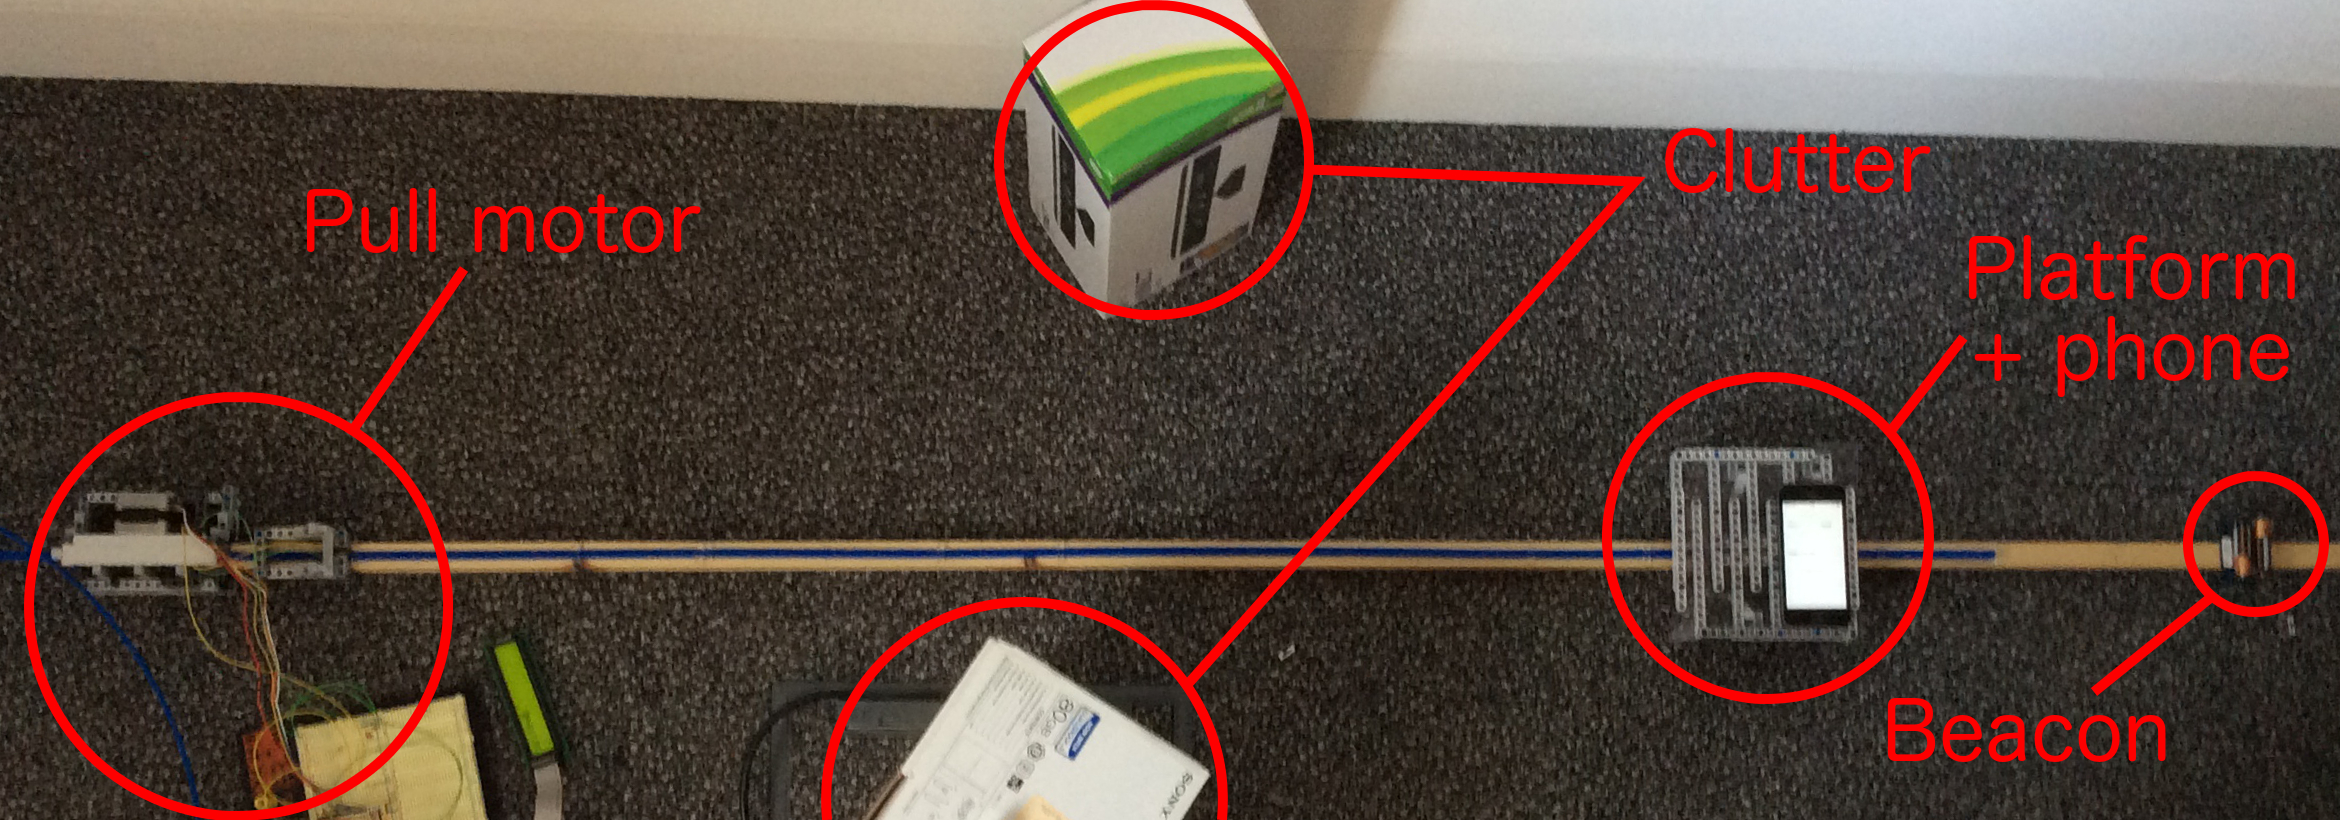
\includegraphics[width=0.8\textwidth]{images/mpi}}
    \end{subfigure}
    \caption{To measure the effect to \mpi, I built a device that pulls a platform with the \device slowly and precisely along a 3 meter path away from a beacon in a cluttered environment. Schematic and photo. The device in the photo is actually shorter than 3 meter, for clarity.}
    \label{fig:rss-pullschematic}
}

\begin{figure}[p]
    \gnuplot{rss}{mpi-combine-channels}{Received signal strength at different distances to a transmitter.}
\end{figure}

\begin{figure}[p]
    \gnuplot{rss}{mpi-split-channels}{Received signal strength at different distances to a transmitter, split out per channel.}
\end{figure}


One of the ways how \mpp can have an influence on RSS, is through \mpi.
\Mpi occurs when a signal propagates via two paths, to be received in the same point.
Depending on the length difference of the two paths, the two signals may strengthen or weaken one another (theoretically making it possible for them to cancel one another out completely).

To explore this effect I built a device that pulls a receiver (an iPhone 5) along a 3 meter track away from a BLE beacon at precisely 1mm/s (\figureref{rss}{pullschematic}).
For each package received, I log the time and the RSS.
Knowing the start-time and start-position, and the speed, I can plot the RSS against the position.
\Figureref{rss}{mpi-combine-channels} clearly shows drops and peaks in the signal that can be attributed to \mpi, however at most distances hugely different RSS values are measured.
Figure \ref{fig:rss-mpi-split-channels} shows the RSS split out by channel, and here we can see that within each channel, the RSS is fairly constant for one location, and each channel shows its own \mpids.

\begin{figure}[p]
    \gnuplot{rss}{mpi-compare}{Top three graphs are RSS of channel 37 during 3 different runs. Bottom graph is RSS of channel 38 during the third run.}
\end{figure}

\newcommand{\correlationtable}[2]{&\cellcolor{#1}#2}
\begin{table}[p]
    \begin{tabular}{ | c | r | c | c | c | c | c | c | c | c | c | }
        \cline{3-11}
        \multicolumn{2}{c |}{} &
        \multicolumn{3}{c |}{run 1} &
        \multicolumn{3}{c |}{run 2} &
        \multicolumn{3}{c |}{run 3} \\
        \cline{3-11}
        \multicolumn{2}{c|}{}
        \h{ch. 37} \h{ch. 38} \h{ch. 39}
        \h{ch. 37} \h{ch. 38} \h{ch. 39}
        \h{ch. 37} \h{ch. 38} \h{ch. 39} \\
        \hline
        \makeandinput{rss}{correlation-table-generated}
    \end{tabular}
    \caption{Pearson-correlation between multiple runs, on the same channel and different channels. Since many data points are involved, there is an extreme high certainty, and the p-value for all measurements is under machine epsilon.}
    \label{tbl:rss-mpi-correlation}
\end{table}

\Figureref{rss}{mpi-compare} shows the RSS for a single channel (37) over three runs (top three graphs), and compares this to channel 38 during the third run.
The same multipath drop pattern is visible in all three runs for one channel, while the other channel has a different pattern.
\Tableref{rss}{mpi-correlation} shows the Pearson correlation (using 1-second means) between different channels and between different runs.
The green cells show the same channel in different runs, and clearly have a much higher correlation than between different channels (the white cells).
This suggests that different channels have their \mpids at different locations, something that is to be expected, since the location of the \mpids is dependent on the wave length, thus on the radio frequency.

\fig{\gnuplot{rss}{mpi-feasibility}{Effect of a small lateral shift of the receiver and small changes in the environment on the RSS}}

It is tempting to try to use the \mpids to improve on positioning via RSS; if the drops can be mapped precisely, the combination of the three individual channels could provide a location with much precision.
For instance, if channel 37 has an RSS of -63dB, channel 38 has -50dB and channel 39 an RSS of -46dB, one could use the information from figure \ref{fig:rss-mpi-split-channels} to find a distance of 1.3m.
One of the challenges here is that the \mpids are very local, and to create fingerprints for a whole room, measurements have to be taken every couple of centimetres at least in all three dimensions.
To illustrate this, figure \ref{fig:rss-mpi-feasibility} shows in purple the original measurements, and in red the measurements taken with the receiver put on the other side of the platform, 4cm to the side of where it was in previous runs.
The same channel in both runs has a Pearson correlation of between 0.83 and 0.88, p-value < machine epsilon, considerably less than the correlation between different runs with the receiver in the same spot.
Even if such a map had been made however, \mpi is dependent on the environment, and even small changes in the environment (movement of objects or people), may invalidate a map.
Figure \ref{fig:rss-mpi-feasibility} shows this effect, purple is the base measurement, green the measurements after some small changes in the environment are made.
This time the correlation coefficient is between 0.48 and 0.66, the same as between different channels in one run.
These two effects mean that simply creating a map of an environment, even for an environment with just small changes, is not feasible, unless additional techniques are developed to combat the described problems.

\fig{
    \begin{subfigure}[b]{0.5\textwidth}
        \gnuplotscale{rss}{mpi-single-rss-10mm}{1cm}{0.55}
    \end{subfigure}
    \begin{subfigure}[b]{0.5\textwidth}
        \gnuplotscale{rss}{mpi-single-rss-100mm}{10cm}{0.55}
    \end{subfigure}
    \begin{subfigure}[b]{0.5\textwidth}
        \gnuplotscale{rss}{mpi-single-rss-400mm}{40cm}{0.55}
    \end{subfigure}
    \begin{subfigure}[b]{0.5\textwidth}
        \gnuplotscale{rss}{mpi-single-rss-1000mm}{100cm}{0.55}
    \end{subfigure}
    \caption{Using average, maximum and median strategies to determine RSS, using different distance intervals}
    \label{fig:rss-mpi-single-rss}
}

The fluctuating RSS value is unhelpful for most positioning methods.
Most positioning methods work by creating a fingerprint map, with RSS values expected to remain more or less the same over time on the same location, and on locations between two spots where fingerprints were collected, the collected RSS values should have a value between those measured in the two surrounding mapping points.
Ideally there is a smooth decrease in RSS with distance; the 6dB decrease per doubling of distance, discussed earlier in this chapter, is used, with different starting points, as an ideal reference line in this section.
Figure \figureref{rss}{mpi-single-rss} shows several strategies we may employ to remove RSS fluctuations.
I take the mean, median and maximum of the received data, over different distance intervals, and compare this to an ideal RSS line.
Taking this over a distance is artificial, since during positioning one does not know the distance travelled; therefore a method should be chosen that works well with any distance.
Figure \ref{fig:rss-mpi-single-rss} shows that both average and median follow one another very closely, with sometimes one and sometimes the other being closer to the ideal line, whereas the maximum fits less nicely but is still has nice smoothing properties.

\section{Orientation}
\label{sec:rss-rot}

The direction in which a user is facing while using a smartphone to position, also has an influence on the RSS.
This may be due to two reasons.
First, the phone itself: rotating the iPhone leads to the antenna being less or more aligned with the signal, and leads to certain parts of the phone blocking the radio signal.
Second, the user's body may either absorb or reflect the signal, leading to signal loss or gain.

\fig{
    \begin{subfigure}[b]{0.55\textwidth}
        \centering{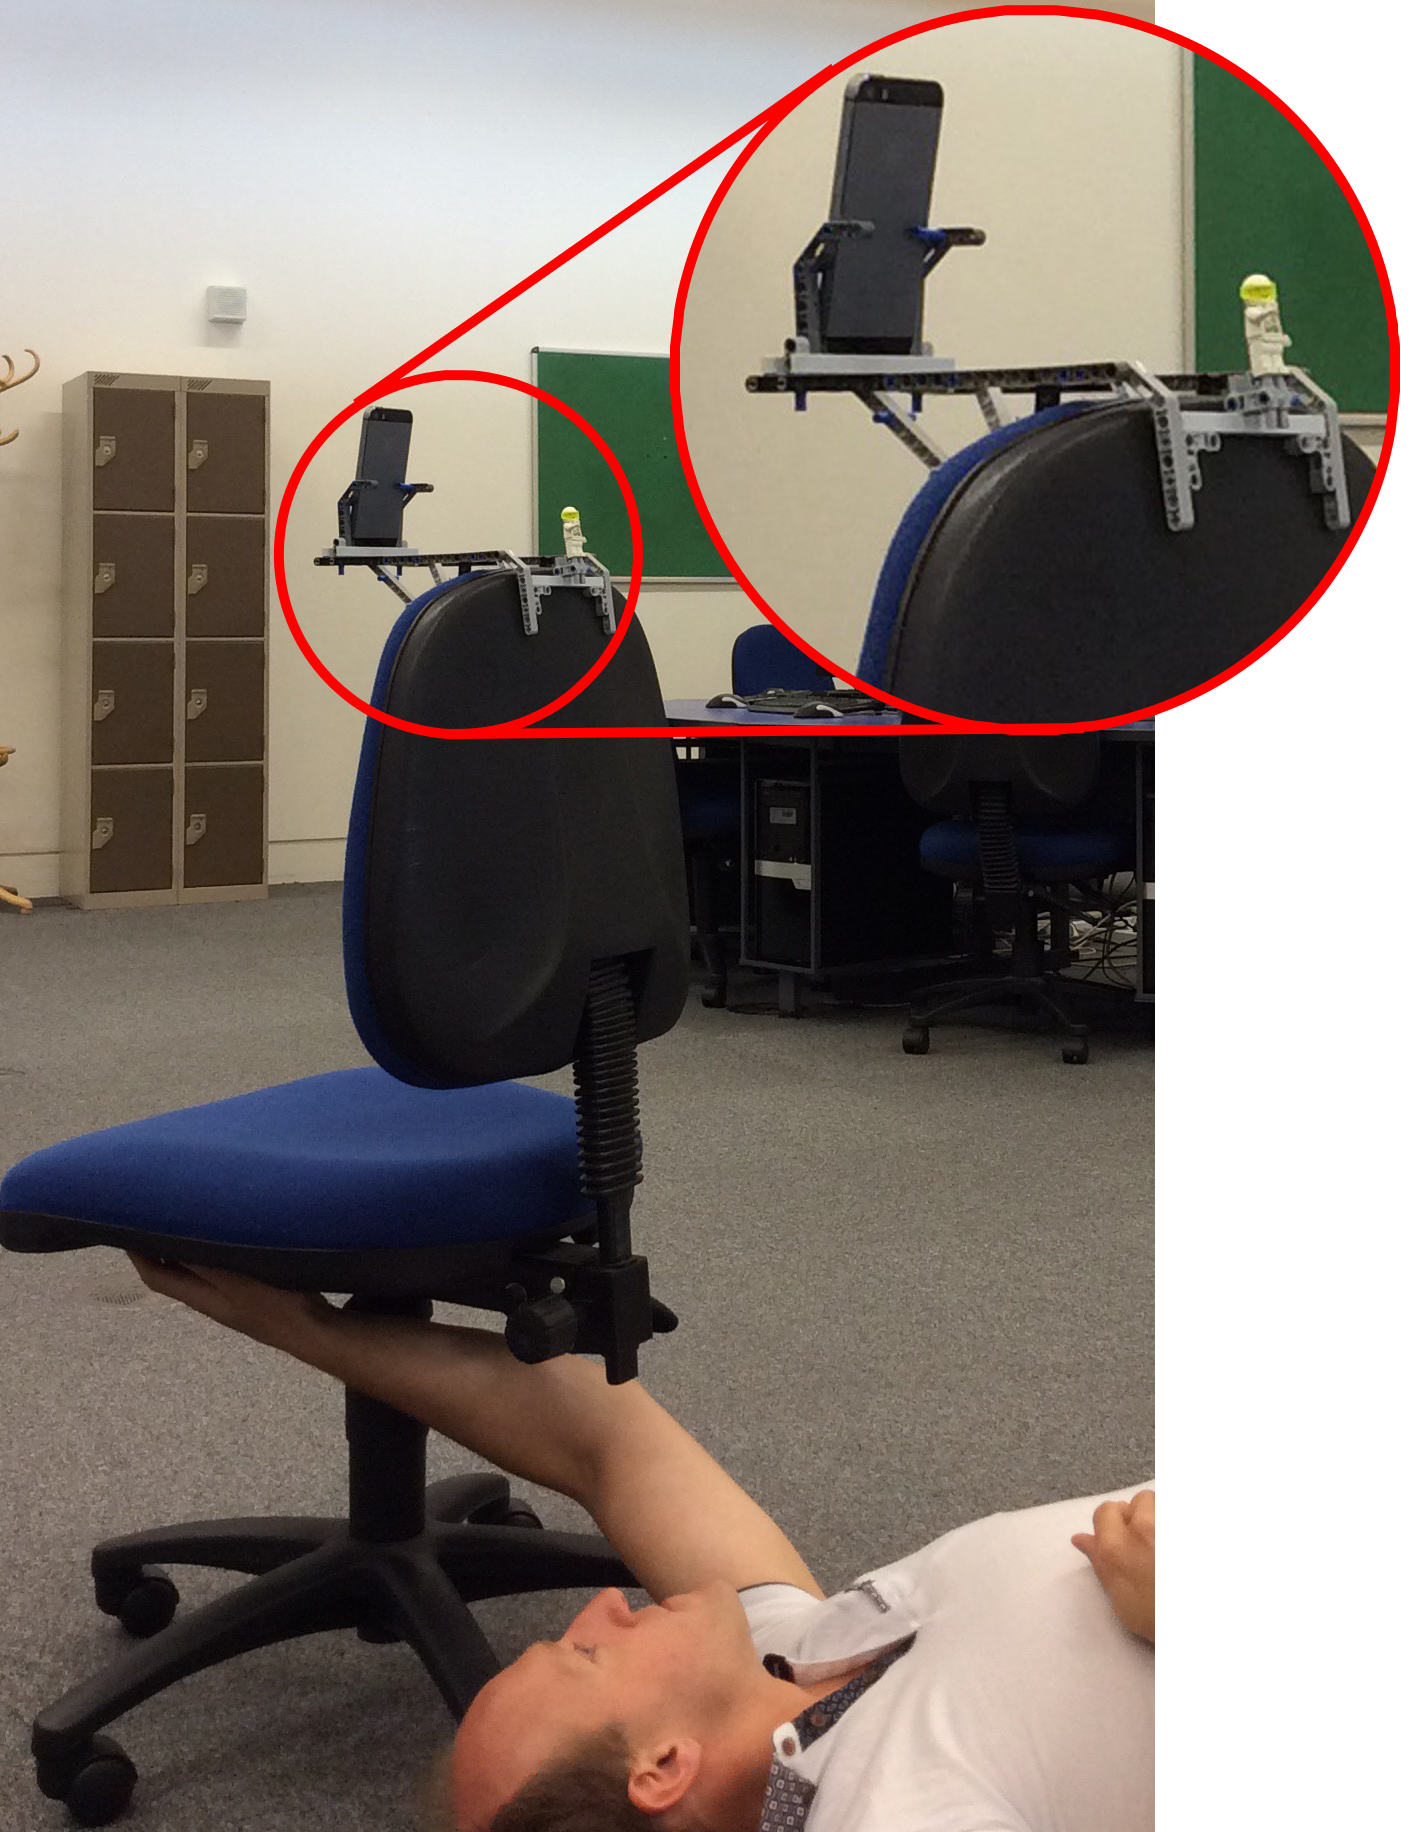
\includegraphics[width=\textwidth]{images/rot-without-body}}
        \caption{without body}
    \end{subfigure}
    \begin{subfigure}[b]{0.45\textwidth}
        \centering{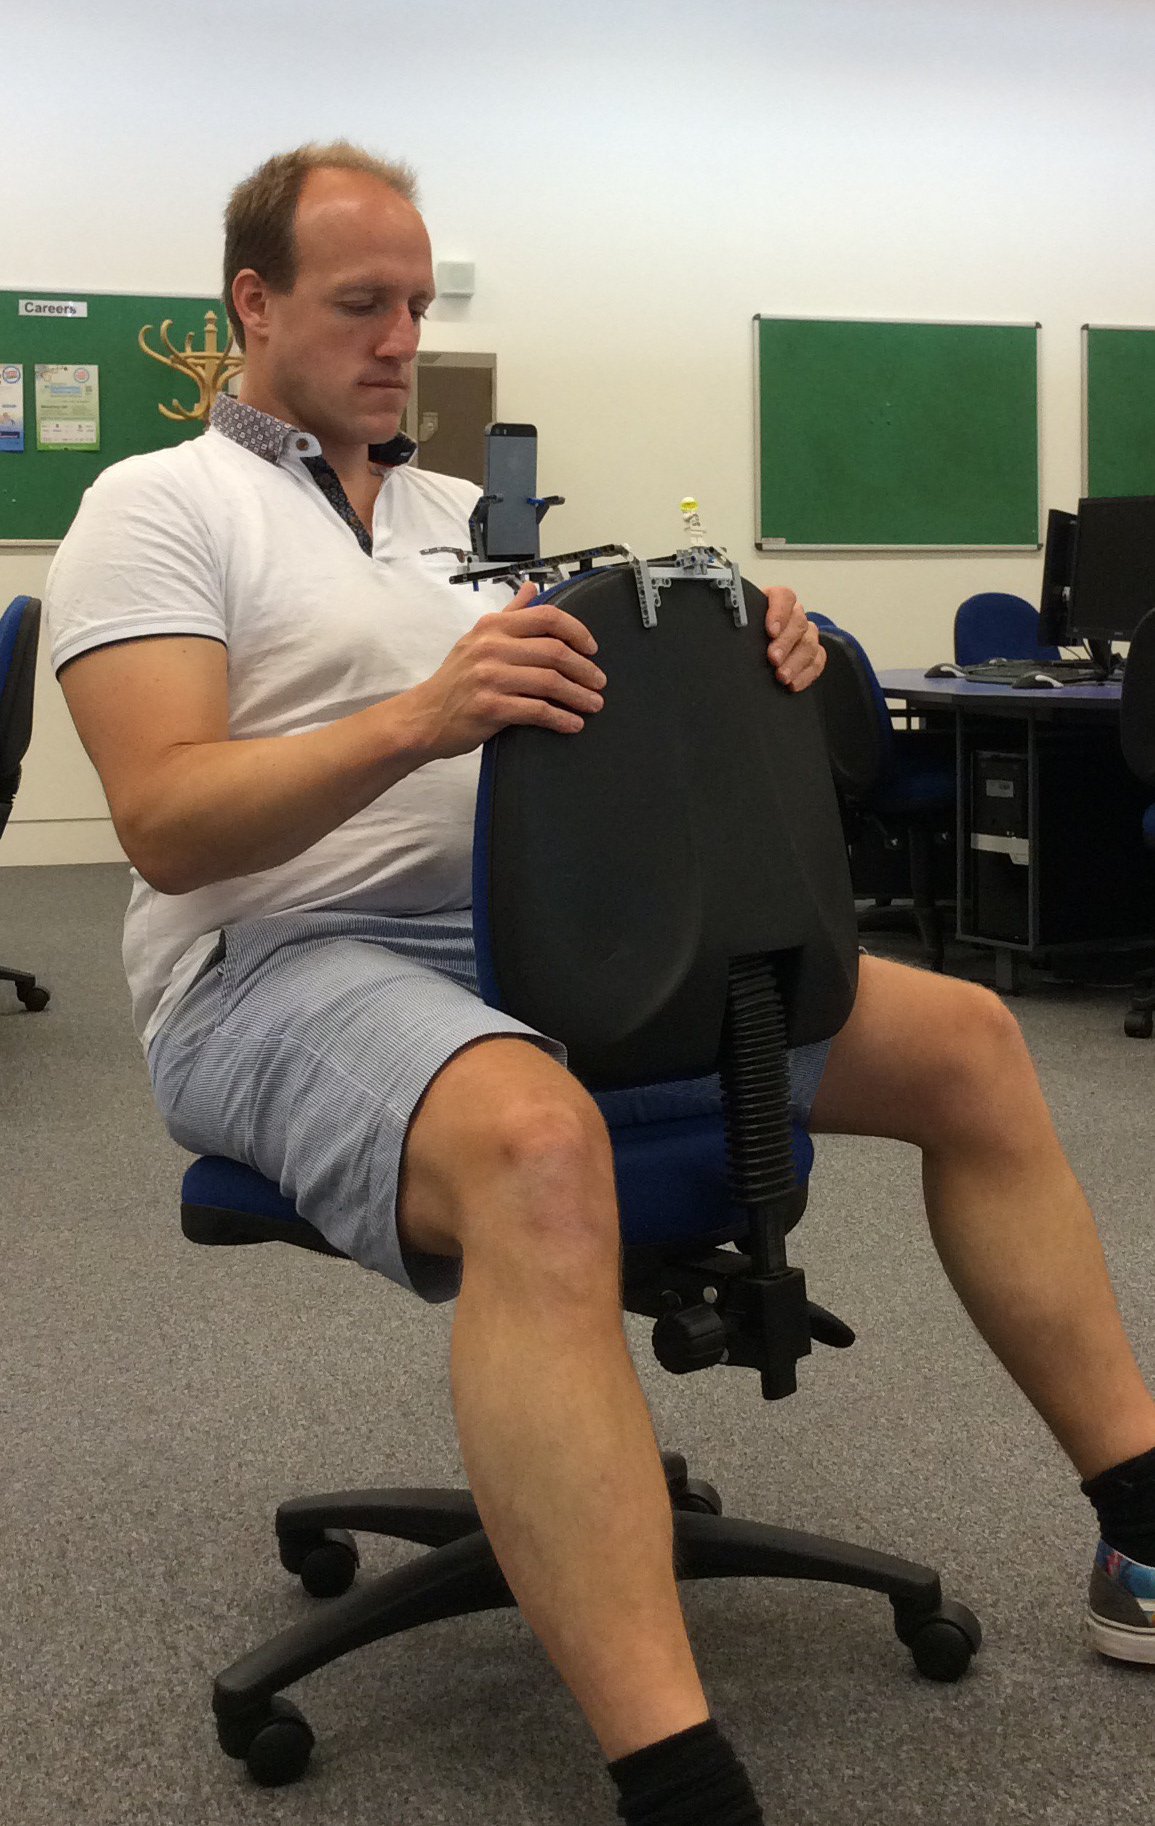
\includegraphics[width=\textwidth]{images/rot-with-body}}
        \caption{with body}
    \end{subfigure}
    \caption{Device used for measuring rotation.}
    \label{fig:rss-rot-device}
}
 

To explore these effects I built a device to rotate the \device around its axis: an small construction was added to the back of an office chair, such that a \device rotates around its axis when the chair rotates (\figureref{rss}{rot-device}).
Using the built-in compass, the heading was recorded together with the RSS.
During measurements an eye was kept on the reading from the compass and no large errors were spotted; small errors in compass accuracy do not have a major influence on the results of this section.
Two measurements were made at each location.
In 300 seconds I rotated the chair 3 $\times$ 360\tdegree, while measuring compass heading, and the RSS for a beacon placed at around 7 meters distance, while lying on the floor under the chair.
Then I sat on the chair with my body around 15 cm from the \device, and did the same 1080\tdegree rotation in 300 seconds.

\fig{
    \begin{subfigure}[b]{0.5\textwidth}
        \gnuplotscale{rss}{rot-grass}{Outside in a field}{0.55}
    \end{subfigure}
    \begin{subfigure}[b]{0.5\textwidth}
        \gnuplotscale{rss}{rot-sw02}{Indoor in a mostly open room}{0.55}
    \end{subfigure}
    \begin{subfigure}[b]{0.5\textwidth}
        \gnuplotscale{rss}{rot-corridor}{Indoor in a corridor}{0.55}
    \end{subfigure}
    \begin{subfigure}[b]{0.5\textwidth}
        \gnuplotscale{rss}{rot-sw02-nolos}{Indoor, transmitter and receiver in different rooms}{0.55}
    \end{subfigure}
    \caption{RSS under rotation, with and without a body present, in different environments.}
    \label{fig:rss-rot}
}

\Figureref{rss}{rot} shows in red the average RSS per 0.5 second, plotted against the direction the phone is facing, while I lie under the chair.
0\tdegree means that the back of phone is the facing the beacon, while at 180\tdegree the screen is facing the beacon.
Since on the iPhone 5 the \wifi/Bluetooth antenna is mounted against the back of the phone, next to the camera and flash\urlref{http://www.ifixit.com/Guide/iPhone+5+Wi-Fi+Antenna+Replacement/10897}{11 June 2014}, I expect reception to be best with that side facing the transmitter.
The blue points show the same rotation with my body on the chair, influencing the signal.
Since I'm facing the screen, at 0\tdegree the \device is between me and the beacon, while at 180\tdegree I am between the beacon and the \device.

\Figureref{rss}{rot}(a) shows that without a body present, both with the back and with the screen facing the beacon, there is optimal reception of -63dB.
Reception generally stays above -70dB, however at two points, around 120\tdegree and 240\tdegree there are large drops to around or even under -80dB, resulting in an RSS difference of 15dB in just 15\tdegree, and a 20dB difference throughout the whole rotation.
These plotted values are already averages, the extremes on different channels are even larger.

In the blue points, the effect of the body is clearly visible, shadowing the signal, resulting in a 20dB drop when between the phone and the beacon, while resulting in a slight boost of the signal when the back of the phone faces the beacon, possibly because of the reflection of the signal by the body.
Also in this case we see 20dB+ drops in the signal strength within a couple of degrees in many spots.

In \figureref{rss}{rot} the experiment is repeated in different environments, generally coming less open from (a) to (d)
In general in (b), (c) and (d) the same patterns as in (a) are visible, that at 180\tdegree the body casts a shadow on the reception, while at 0\tdegree a slight boost of signal can be seen when there is a body behind the device.
The effect is arguably smaller in the more cluttered environments, possibly because reflections result in multiple paths the signal can take around the body.
All environments show some drop orientations, where the RSS drops by 10-20dB within a couple of degrees.

\section{People moving through the room}
\label{sec:rss-busyroom}

\fig{\gnuplot{rss}{drawmeetingroom}{Schematic of meeting room in lunch setting.}}
In order to investigate how people and objects moving around a room influence RSS, 6 beacons were placed in a meeting room, together with an iPad mini as receiver on a table (\figureref{drawmeetingroom}), while a standing lunch was taking place.
All tables and chairs were moved to the side before the start of measurements.
\Figureref{rss}{busyroom} shows the RSS over time for six beacons, and how many packets of were received on each channel; the other beacons show similar data.
Beacons 1 and 2 were placed in the ceiling left and right of the receiver, beacons 3 and 4 on the floor.
Beacon 5 was placed just behind the receiver, and beacon 6 across the room, both at table height.
Even though beacon 6 was furthest away, the highest RSS of all beacons is received from this one; this may be because it is in front of the receiver on a direct line of sight.

\begin{figure}[p]
    \begin{subfigure}[b]{0.5\textwidth}
        \gnuplotscale{rss}{busyroom-0x12}{Beacon 1 (left side ceiling)}{0.55}
    \end{subfigure}
    \begin{subfigure}[b]{0.5\textwidth}
        \gnuplotscale{rss}{busyroom-0x10}{Beacon 2 (right side ceiling)}{0.55}
    \end{subfigure}
    \begin{subfigure}[b]{0.5\textwidth}
        \gnuplotscale{rss}{busyroom-0x08}{Beacon 3 (left side floor)}{0.55}
    \end{subfigure}
    \begin{subfigure}[b]{0.5\textwidth}
        \gnuplotscale{rss}{busyroom-0x06}{Beacon 4 (right side floor)}{0.55}
    \end{subfigure}
    \begin{subfigure}[b]{0.5\textwidth}
        \gnuplotscale{rss}{busyroom-0x14}{Beacon 5 (near)}{0.55}
    \end{subfigure}
    \begin{subfigure}[b]{0.5\textwidth}
        \gnuplotscale{rss}{busyroom-0x13}{Beacon 6 (across)}{0.55}
    \end{subfigure}
    \caption{RSS and the number of packets seen for six beacons during different room occupation.}
    \label{fig:rss-busyroom}
\end{figure}

Five periods were marked using a wristwatch, these are shown in the graphs:
\begin{itemize}
    \item Period 1 (12:41-12:59): The lunch is being built up, occasionally people enter and leave the room, most of the time there are one or two people in the room.
        The door to the room is open.
    \item Period 2 (12:59-13:27): The room fills up with people, people move around, in the first half of the period there are between 15 and 20 people in the room, after which the room slowly empties.
        At the end of the period the last group of 3 people leave, and they close the door.
    \item Period 3 (13:27-13:44): The room is empty.
    \item Period 4 (13:44-13:47): Without moving any beacons or receivers, the furniture in the meeting room is put back to meeting room position, the door is closed again afterwards.
    \item Period 5 (13:47-13:52): The room is empty.
\end{itemize}

The two periods with an empty room, 3 and 5, are characterised in the graphs in \figureref{rss}{busyroom} by relatively low variance in RSS per channel, whereas period 2, when a lot of people are moving around, shows high variance, with periods 1 and 4 being somewhere in between.
The differences between period 3 and 5 show the influence of the furniture on the RSS, where major differences between period 1 and 3 are most likely caused by the door being open or closed.
This latter effect is especially clear with beacons 1 and 3, which are respectively in the ceiling and on the floor behind the door.

The beacons broadcast at 10Hz\footnote{The beacons were set to broadcast at 10Hz, however measurements actually show a 105ms delay between packets, so 9.5Hz is more accurate. This small discrepancy does not influence the conclusions in this section however.}, however in no period more than 6 advertising packets per second are received on average.
In the next section I look into packet loss in more detail, but it is interesting to note the large differences in packet loss between channels, and between periods.
It shows that when the RSS drops below -80dB, less (or hardly any sometimes) packets are received.

\section{Packet loss}
\label{sec:rss-packet-loss}
According to the \BTspec, an advertising packet should be sent on all three advertising channels within a short time.
This means that a beacon advertising at 10Hz (the beaconing rate) sends 10 packets per second on each of the three channels, heaving a 100ms \define{beaconing interval}.

A \device listening for advertisements typically listens on one channel at a time, but switches quickly between the channels, since (as previous sections show) not all devices can be received equally well on all channels at all times.
If a \device were to switch channels at exactly the same moment as a beacon, it could, in theory, receive all 30 packets, however since these two are normally not synchronised, one can expect a 1/3 chance that a \device is listening on the channel the beacon is transmitting on, resulting in a maximum of 10 receivable packets per second\footnote{Inspection of the packet logs for the experiments done in this section, shows that sometimes two packets on different channels are received in very quick succession (much less than 100ms delay), however this happens even more often for two packets on the same channel, suggesting that either the beacons sometimes send at a different rate, or (more likely in my opinion) the timestamp put on the packet by the OS may be off by a couple of tens of ms. This suggests however that the \device never receives more than one packet that was sent as part of the same beacon interval.}.

However there may be many reasons why fewer than 10 packets are received.
Either a packet may, because of \mpi, orientation or signal blocking, not be receivable at the location of the \device, or there may be interference from other transmitters sharing the same frequency, there may have been general radio interference, or the \device may not have been listening at the right time (it was switching channels half way the packet, the \device may have small periods it does not listen to save energy, or possibly the OS discards some packets).
When I talk about packet loss, I refer to the difference between the number of packets sent on each channel, and the number of packets received in total; so if 9 packets are received per second from a 10Hz beacon, there is 10\% packet loss.

As mentioned in \sectionref{rss}{smartphone}, an iOS device misses more packets if \BLE listening is active for a longer time.
To counter this, I restart BLE listening every 10 seconds in all experiments; I do not see increased packet loss at the time of restarting.

If packets are not received consistently, this may impact the positioning ability.
There is no way for the device to know whether a beacon was not observed because it is out of range, or because the packets sent by the beacon were lost.
In my experiments beacons transmit at 10Hz.
Beacons may be set to advertise at a lower rate in order to save energy; these beacons are obviously more easily missed if packets are lost.

To investigate packet loss I used a single beacon transmitting at 1Hz.
The measurements were done outside in a field, with no other known transmitters nearby, distance between beacon and \device 15 centimetres.
In 136 seconds, 12 times 1 packet was not received, 7 times 2 packets, and twice 3 packets in a row, resulting in a total of 32 lost packets, 23.5\%.

\fig{\gnuplot{rss}{packet-loss}{Packet loss for different numbers of beacons.}}
Next I repeated the experiment with first a single beacon set to transmit at 10Hz\footnote{As discussed previously, the actual transmit frequency of these beacons is 9.5Hz. In the text I will continue to call them 10Hz beacons, because 10Hz and 100ms are easier to reason with than 9.5Hz rate and 105ms intervals, and because 10Hz is the setting the beacons were set to. All packet loss calculations however in this section have been done with the actual rate of 9.5Hz.}, then multiple beacons, all set to 10Hz, all within a 20cm radius of the \device.
Each test was ran for one minute; the results can be seen in \figureref{rss}{packet-loss}.
It shows a packet loss of between 27 and 38\%, with a generally a higher packet loss for a larger number of beacons.
This can be explained because packets from different beacons may collide when sent at the same moment.

\begin{table}
    \begin{tabular}{r | c | c | c | c | c | c | c | c | c | c |}
        & \multicolumn{10}{c |}{listening time in transmission intervals} \\
        \makeandinput{rss}{packet-loss-generated}
    \end{tabular}
    \caption{Expected chance that not all beacons have been observed at different listening intervals, with a random packet loss of 38\%.}
    \label{tbl:rss-packet-loss}
\end{table}

\begin{table}
    \begin{tabular}{r | c | c | c | c | c | c | c | c | c | c |}
        & \multicolumn{10}{c |}{listening time in transmission intervals} \\
        \makeandinput{rss}{packet-loss-empirical-generated}
    \end{tabular}
    \caption{Measured chance that not all beacons have been observed at different listening intervals.}
    \label{tbl:rss-packet-loss-empirical}
\end{table}

For positioning it is important to know how long one has to listen to be reasonably sure that, if a beacon has not been observed, it can not be observed in that location.
\Tableref{rss}{packet-loss} shows the chance of not observing a beacon that is observable, if there is a random 38\% chance that a packet is lost, at different listening intervals, where listening intervals are measured in beacon intervals, i.e.\ a listening interval of 3 means 300ms when 10Hz beacons are used.
\Tableref{rss}{packet-loss-empirical} shows in which percentage of the measured cases we failed to observe all beacons; it shows that although the packet loss with 20 beacons is the same 38\%, the chances of missing at least one beacon in multiple listening intervals are much higher.
The reason for this is that not each package has the same chance of being missed (something that we also see in \figureref{rss}{busyroom}, where packages from some beacons are lost more often than others).
This shows that a long listening interval is needed for a high certainty that all beacons have been received at least once.

The tests above were done in an area with minimal additional radio interference.
Looking at a more noisy environment, such as the one of \sectionref{rss}{busyroom}, there is 59\% packet loss, and even after 5.25 seconds, 50 beacon-interval at 9.5Hz, in 1\% of cases not all beacons have been observed.
This can probably be attributed to interference from \wifi and other Bluetooth devices, as well as there not always being a line-of-sight between beacon and \device.
